\documentclass{article}[18pt]
\usepackage{../../../format}
\lhead{A Level Physics - Nuclear Physics}

%File specific preamble
%Diagrams
\usetikzlibrary{decorations, decorations.text,positioning,quotes,arrows.meta,decorations.markings,3d,shapes,decorations.pathmorphing}
\pgfplotsset{width=10cm,compat=1.9}

\usetikzlibrary{calc,quotes,angles}
\tikzstyle{arrow} = [thick,->,>=stealth]

%Proper paragraph formatting
\setcounter{secnumdepth}{4}
\titleformat{\paragraph}
{\normalfont\normalsize\bfseries}{\theparagraph}{1em}{}
\titlespacing*{\paragraph}
{0pt}{3.25ex plus 1ex minus .2ex}{1.5ex plus .2ex}

\begin{document}
\begin{center}
\underline{\huge Radioactivity}
\end{center}
\section{Rutherford Scattering}
\subsection{The plum pudding model}
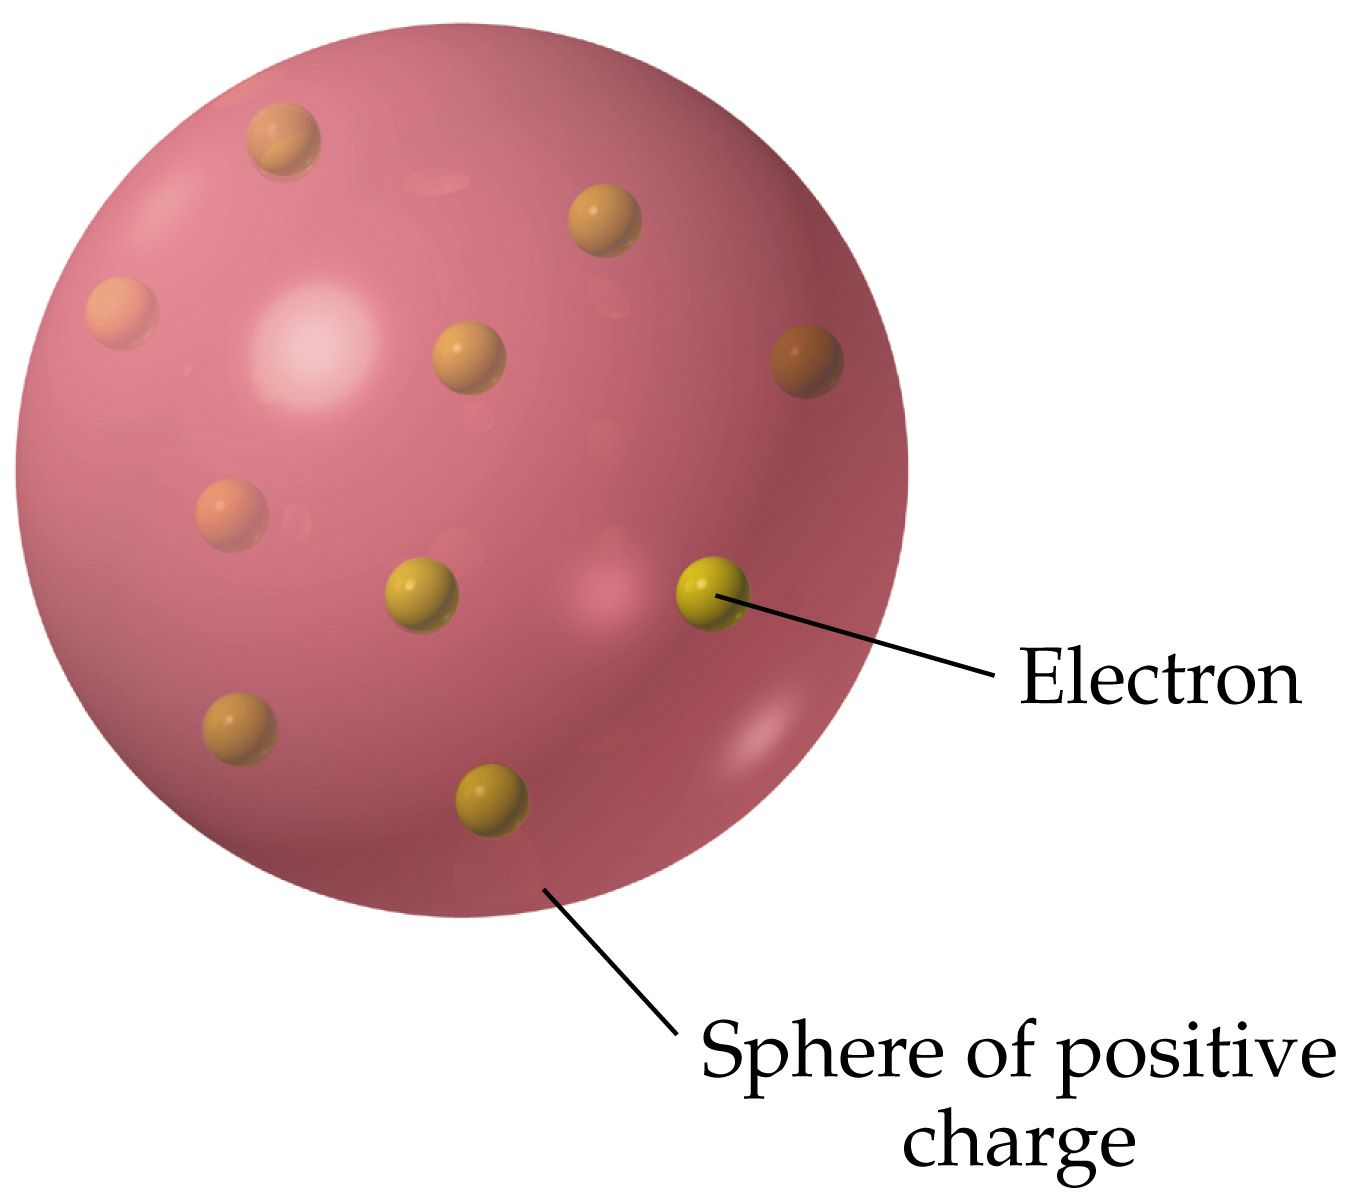
\includegraphics[width=3cm] {plum.jpg}  
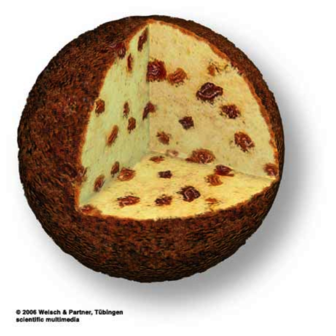
\includegraphics[width=3cm] {Plumpudding.png}
\\
The plum pudding model was the initial model of the atom, stating a sphere of positive charge with electrons embedded into it.
\subsection{Rutherford's experiment}
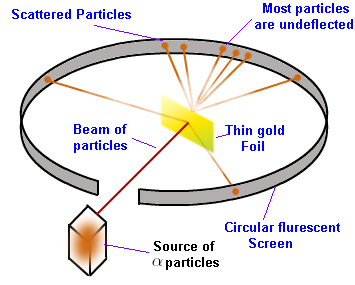
\includegraphics[width=6cm] {scatter.png}\\
Rutherford's experiment involved firing a beam of alpha particles at gold foil and measuring the paths of particles from the foil.
\begin{itemize}
\item Gold was used as it was expected to have a large nucleus
\item The screen fluoresces when collided with
\item This showed the atom was mostly empty space with a positive nucleus
\end{itemize}
\subsubsection{Results}

\begin{figure}[h]
    \centering
    \begin{minipage}{0.45\textwidth}
        \centering
        
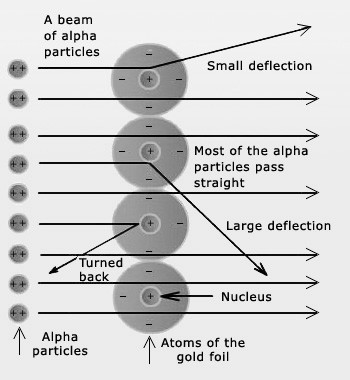
\includegraphics[width=6cm]{foil.jpg}  
    \end{minipage}\hfill
    \begin{minipage}{0.45\textwidth}
        \centering
\begin{tabularx}{\textwidth}{|X|X|}
\hline
Observation&Explanation\\
\hline
Most electrons pass all the way through&Atoms are mostly empty space\\
\hline
Some are deflected&The atom has a positive centre\\
\hline
Some are deflected by significant angles&The positive charge is condensed in a small area\\
\hline
\end{tabularx}
    \end{minipage}
\end{figure}
\subsection{Estimating the size of the nucleus}  
\subsubsection{Closest approach method}
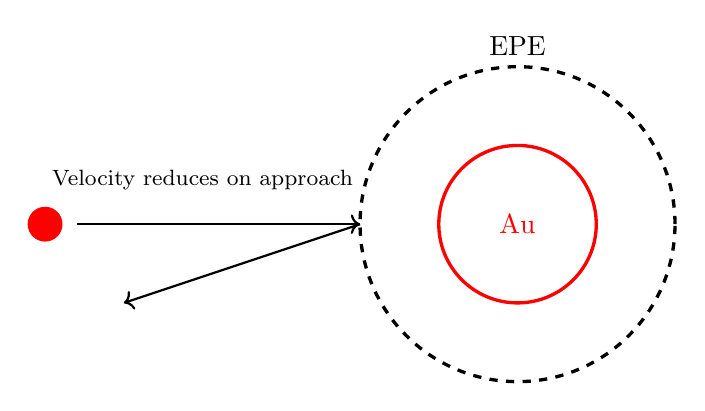
\begin{tikzpicture}
\filldraw[color=red, fill=red, very thick](0,0) circle (0.2);
\draw[thick, ->,black] (0.4,0) -- (4,0) node[above,yshift=0.3cm,xshift=-2cm] {\footnotesize{Velocity reduces on approach}};
\draw[color=red, very thick](6,0) circle (1) node[] {Au};
\draw[color=black, very thick,dashed](6,0) circle (2) node[above,yshift=2cm] {EPE};
\draw[thick, ->,black] (4,0) -- (1,-1);
\end{tikzpicture}\\
\\
KE=EPE
$$8.0\times10^{-13}=\frac{1}{4\pi\epsilon_0}\times\frac{Q_{Au}}{r}\times Q_{\alpha}$$
$$r=4.55\times10^{-14}$$
\subsubsection{Estimate from scattering data}
\begin{itemize}
\item About $\frac{1}{10,000}$ deflected through more than 90\degree
\item Foil had n layers of atoms
\end{itemize}
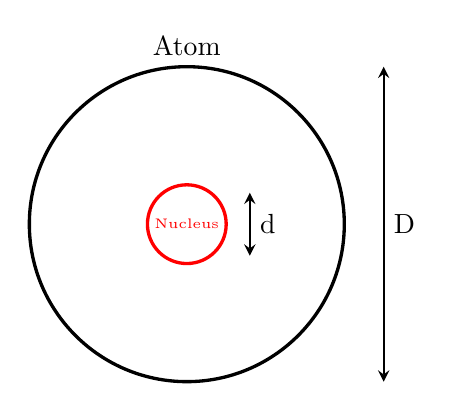
\begin{tikzpicture}
\draw[thick, stealth-stealth,black] (6.8,-0.4) -- (6.8,0.4) node[right,midway] {d} ;
\draw[color=red, very thick](6,0) circle (0.5) node[] {\tiny{Nucleus}};
\draw[color=black, very thick](6,0) circle (2) node[above,yshift=2cm] {Atom};
\draw[thick, stealth-stealth,black] (8.5,-2) -- (8.5,2) node[right,midway] {D};
\end{tikzpicture}\\
$$\frac{\frac{1}{4}\pi d^2}{\frac{1}{4}\pi D^2}=\frac{d^2}{D^2}=\frac{1}{10,000n}$$
$n=10^4$ layers
$$\frac{d^2}{D^2}=\frac{1}{10,000\times1\times10^4}$$
$$d=\frac{D}{10,000}$$
\newpage
\section{Radioactive materials}
\subsection{Sources of background radiation by most common}
\begin{enumerate}
\item Air (e.g. radon gas)
\item Medical
\item Ground and buildings
\item Food and drink
\item Cosmic rays
\item Nuclear weapons
\item Air travel
\item Nuclear power
\end{enumerate}
\subsection{Geiger M\"{u}ller tube}
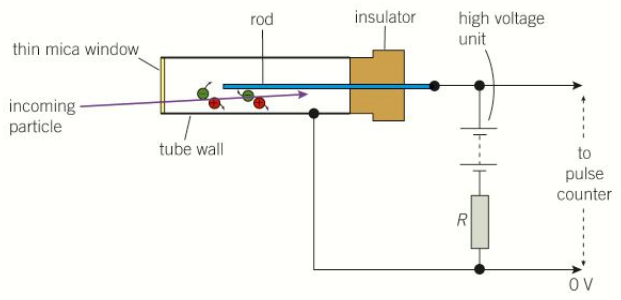
\includegraphics[width=10cm]{geiger.png}\\
When a particle of ionising radiation enters the tube, the particle ionises the gas atoms along its track. The negative ions are attracted to the rod and the positive ions to the wall. These ions cause further ionisation, creating enough ions for a current to flow. A pulse of charge passes round the circuit through resistor R, causing the voltage pulse across R which is recorded as a single count by the pulse counter\\
\\
The dead time of the tube, the time taken to regain its non conducting state after an ionising particle enters it, is typically of the order of 0.2ms.\\
\section{Radioactive decay}
\begin{tabularx}{\textwidth}{|c|X|X|X|}
\hline
&Alpha&Beta&Gamma\\
\hline
Nature&2 Protons+2 Neutrons&High speed electron or positron&High energy photon\\
\hline
Range&Up to 10cm&Up to 1m&Infinite\\
\hline 
Deflection in a magnetic field&Deflected&Opposite direction to $\alpha$ particles and more easily deflected&Not deflected\\
\hline
Absorption&Paper&Aluminium&Lead \\
\hline
Ionisation&$10^4$ ions per mm&100 ions per mm&Very weak ionising effect\\
\hline
Energy of each particle&Constant for a given source&Varies up to a maximum for a given source&Constant for a given source\\
\hline
\end{tabularx}
\newpage
\subsection{$\alpha$ Decay}
$$^{238}_{92}U\rightarrow^4_2\alpha+^{234}_{90}Th$$
\subsection{$\beta^-$ Decay}
Neutron to proton and $\beta^-$ particle
$$^{14}_6C\rightarrow^0_{-1}\beta+^{14}_7N$$
\subsection{$\beta^+$ Decay}
Proton to neutron and $\beta^+$
\subsection{Electron Capture}
Proton+Electron$\rightarrow$ Neutron
\subsection{Gamma Emission}
No change to the structure of the nucleus.\\
Often follows alpha or beta emission. Daughter nucleus can be in an excited state. It emits gamma radiation as it returns to its ground state.
\subsection{NZ Plot}
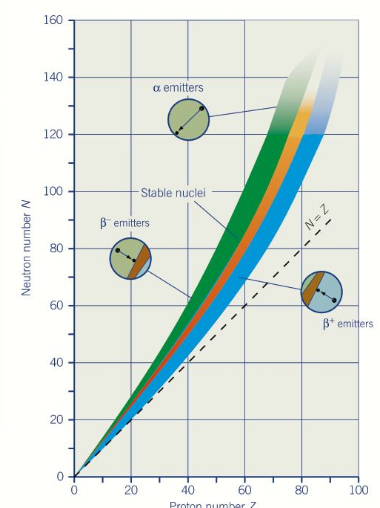
\includegraphics[width=5cm]{nz_plot.png} 
\subsection{Half life}
The half life of a radioactive substance is the time taken for half the atoms in the sample to decay.
$$\textrm{The rate of decay}\propto\textrm{The number of nuclei left}$$
$$-\frac{\Delta N}{\Delta t}\propto N$$
The LHS of this equation is called the activity and has units Bq
$$-\frac{\Delta N}{\Delta t}=\lambda N$$
The solution to this equation
$$N=N_0e^{-\lambda t}$$
This can also be written as:
$$\frac{N}{N_0}=e^{-\lambda t}$$
\subsubsection{Linking the formula to half life}
After a time, t=$T_{\frac{1}{2}}$ the fraction remaining is 0.5.
$$0.5=e^{-\lambda t}$$
$$ln(2)=\lambda t$$
$$t=\frac{\ln(2)}{\lambda}$$
$\lambda t$ is a "Pure Number". As long as the same units are used for both, you can use any unit of time.\\
\\
$\lambda$ is the fraction of nuclei decaying per unit time or the probability of an individual nucleus decaying per second.\\
As N is proportional to Activity, Mass and Count Rate N can be replaced with any of these in the formula.
\section{Nuclear radius}
\subsection{High energy electron diffraction}
When a beam of high energy electrons is directed at a thin solid sample of an element they are diffracted by the nuclei of the atoms.\\
The electrons are diffracted by the nuclei because of their de Broglie wavelength, this is approximately equal to the radius of the nuclei. The detector measures the number of electrons per second at different angles.\\
The scattering of the beam of electrons occurs due to the charge, this causes intensity to decrease as angle increases.\\
The minimum on the graph can then be used to find the radius of the nucleus.
\subsection{Dependence of nuclear radius on nucleon number}
It can be shown that radius depends on mass according to:
$$\mathlarger{R=r_0A^{\frac{1}{3}}}$$
Where $r_0$ is the constant 1.05fm\\
\\
The graph of $\ln(R)$ against $\ln(A)$ gives a line with gradient $\frac{1}{3}$ and y intercept equal to $\ln(r_0)$\\
\\
The graph of R against $A^{\frac{1}{3}}$ gives a straight line through the origin with gradient $r_0$\\
$$V=\frac{4}{3}\pi R^3=\frac{4}{3}\pi(r_0A^{\frac{1}{3}})^3=\frac{4}{3}\pi r_0^3A$$
As $\textrm{Density}=\frac{\textrm{Mass}}{\textrm{Volume}}$
$$\textrm{Density}=\frac{Au}{\frac{4}{3}\pi r_0^3A}=\frac{1u}{4\pi r_0^3}=\frac{1.661\times10^{-27}}{\frac{4}{3}\pi(1.05\times10^{-15})^3}=3.4\times10^{17}kgm^{-3}$$
\newpage
\section{Radioactive isotopes in use}
\subsection{Radioactive dating}
\subsubsection{Carbon dating}
Carbon-14 is used for carbon dating, this has a half life of 5570 years, meaning that there is very little decay while a plant is alive. However once the tree has died, the percentage of carbon-14 reduces as it decays. Because activity is proportional to the number of atoms still to decay, measuring the activity of the dead sample allows its age to be calculated.
\paragraph{Example}
\textit{A sample of dead wood is found to have an activity of 0.28Bq. An equal mass of living wood is found to have an activity of 1.3Bq.Calculate the age of the sample\\
\\
The half life of carbon-14 is 5570 years }\\
\\
Calculate the half life in seconds
$$T_{\frac{1}{2}}=5570\times365\times24\times3600=1.76\times10^{11}s$$
Calculate the decay constant using the formula on the formula sheet
$$\lambda=\frac{\ln(2)}{1.76\times10^{11}}$$
Use the formula $A=A_0e^{-\lambda t}$
$$0.28=1.8e^{-\lambda t}$$
Rearrange to find $\lambda t$
$$e^{-\lambda t}=\frac{0.280}{1.30}=0.215$$
$$\lambda t=1.535$$
Rearrange and substitute in $\lambda$ to find t
$$t=\frac{1.535}{\lambda}=\frac{1.535}{3.96\times10^{-12}}=3.88\times10^{11}s=12300 \ \textrm{years}$$
\subsubsection{Argon dating}
$$^{40}_{19}K+^0_{-1}e\rightarrow^{40}_{18}Ar+\nu_e$$
The effective half-life of the decay of $^{40}_{19}K$ is 1250 million years. The age of the rock can be calculated by measuring the proportion of argon-40 to potassium-40.\\
\\
$^{40}_{19}K$ also decays to $^{40}_{20}Ca$. This process is eight times more probable than electron capture. This means that if there was one argon atom for every N potassium atoms, there would originally be N+9 potassium atoms, eight decaying to Calcium and one decaying to argon.
\paragraph{Example}
\textit{Suppose for every 4 potassium-40 atoms present a certain rock now mas 1 argon-40 atom, what is the age of the sample?}\\
\\
Find the values of $N$ and $N_0$ 
$$N=4 \qquad N_0=4+9=13$$
Substitute these values into $N=N_0e^{-\lambda t}$
$$4-13e^{-\lambda t}$$
Rearrange to find t 
$$t=\frac{-\ln\frac{4}{13}}{\lambda}$$
Substitute $\frac{\ln(2)}{T_{\frac{1}{2}}}$ for $\lambda$
$$t=\frac{-\ln(\frac{4}{13})}{0.693}T_{\frac{1}{2}}$$
Substitute in the known value of the half life of potassium
$$1.7\times T_{\frac{1}{2}}=2120 \  \textrm{million years}$$
\subsection{Radioactive tracers}
A radioactive tracer follows the path of a substance through a system. These should:
\begin{itemize}
\item Have a half life stable enough for the necessary measurements to be made and short enough to decay quickly after use
\item Emit $\beta$ radiation of $\gamma$ radiation so it can be detected outside the flow path
\end{itemize}
\subsection{Industrial uses}
\subsubsection{Engine wear}
The rate of wear of a piston ring can be measured by fitting a ring that is radioactive. This causes transfer of radioactive atoms from the ring to the engine oil, which can then be measured
\subsubsection{Underground pipe leaks}
Radioactive tracer is injected in the flow, A detector at the surface measures the leakage
\subsubsection{Investigating the uptake of fertilisers by plants}
The fertiliser is a $\beta^-$ emitter and so can be measured in the leaves.
\subsubsection{Thickness monitoring}
The thickness of continuous materials can be measured by placing a $\beta$ emitter and detector on either side of the material. This allows materials such as foil to have a uniform thickness.
\subsubsection{Power sources for remote devices}
Satellites, weather sensors etc can be powered using a radioactive isotope in a thermally insulated sealed container which absorbs all the radiation emitted by the isotope. A thermocouple attached to the container produces electricity of the container being warm.
\section{Inverse square law for $\gamma$}
$$\textrm{Intensity}\propto\frac{1}{d^2}$$
$$I=\frac{k}{x^2}$$
\section{Liquid drop model}
This uses a water droplet as a model for the nucleus\\
Molecules of water are held together by short range forces - similar to the nucleus\\
\\
It can become more stable by splitting into two smaller spherical droplets\\
\\
When a nucleus absorbs a neutron, oscillations can be set up which cause elongation.



\end{document}
